\section{Model trained on the synthetic data}

The final model from Section \ref{subsec:finalmodel} was evaluated on the testing dataset and has achieved 73.00 \% accuracy, 73.52 \% precision and 73.00 \% recall. 

From the confusion matrix in the Figure \ref{img:confmatrixsyn} we can see that the model has the biggest problem distinguishing between galaxy and streak (more than 30 cases). This is caused by the fact that elliptical galaxies with a high degree of ellipticity resemble streaks and even professionals wouldn't be able to tell the difference just from one image. Another prevalent problem is the misclassification of streaks as points (10 cases) and points as cosmic rays (13 cases). In the Figure \ref{fig:wrongsyn} we show some examples of wrongly classified images, where we can see that these problems are usually caused by small streaks that resembled points (\ref{fig:streakpointmis3}), and points with small fwhm which caused them to look like spots (\ref{fig:pointcosmicmis3}).   

\begin{figure}[h]
    \centering
    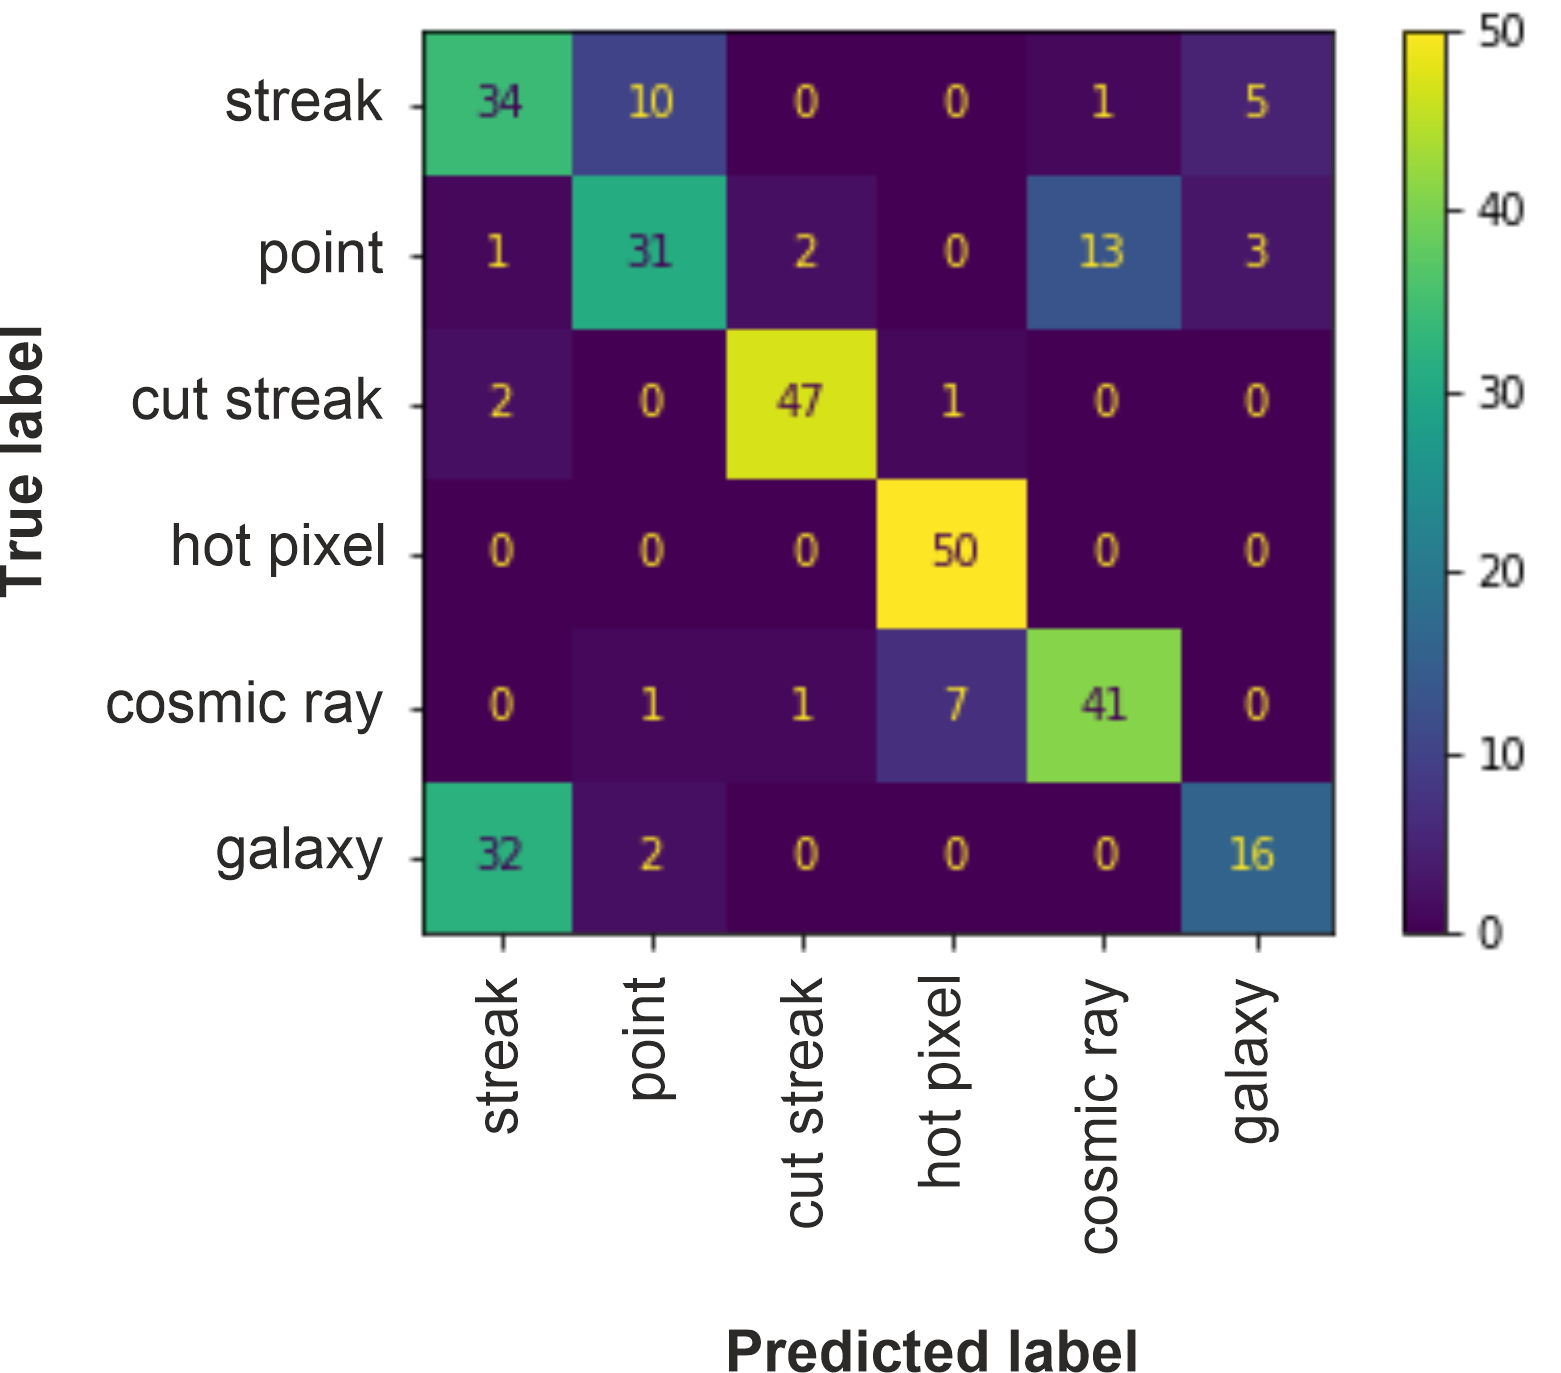
\includegraphics[width=.5\textwidth]{images/confusionmatrix51.png}
    \caption{Confusion matrix from the testing of the final model trained only on synthetic data.}
    \label{img:confmatrixsyn}
\end{figure}

\begin{figure}[!h]
\centering
    \begin{subfigure}[t]{.23\textwidth}
        \centering
        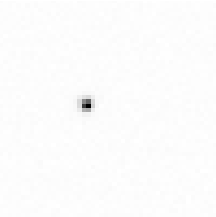
\includegraphics[width=\textwidth]{images/wrongImage8.png}
        \caption{}
        \label{fig:pointcosmicmis3}
    \end{subfigure}
    \begin{subfigure}[t]{.23\textwidth}
        \centering
        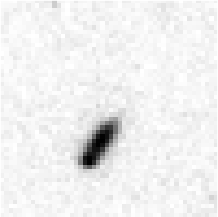
\includegraphics[width=\textwidth]{images/wrongImage18.png}
        \caption{}
    \end{subfigure}
    \begin{subfigure}[t]{.23\textwidth}
        \centering
        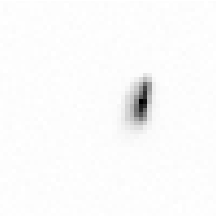
\includegraphics[width=\textwidth]{images/wrongImage34.png}
        \caption{}
    \end{subfigure}
    \begin{subfigure}[t]{.23\textwidth}
        \centering
        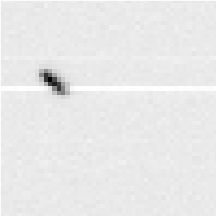
\includegraphics[width=\textwidth]{images/wrongImage48.png}
        \caption{}
        \label{fig:streakpointmis3}
    \end{subfigure}

    \caption[Wrongly classified images on the model that trained only with synthetic data.]{Wrongly classified images on the model that trained only with synthetic data. (a) A point misclassified as a cosmic ray, (b) A galaxy misclassified as a streak, (c) A streak misclassified as a galaxy, (d) A streak misclassified as a point. }
    \label{fig:wrongsyn}
\end{figure}


